\documentclass[]{article}
\usepackage{lmodern}
\usepackage{amssymb,amsmath}
\usepackage{ifxetex,ifluatex}
\usepackage{fixltx2e} % provides \textsubscript
\ifnum 0\ifxetex 1\fi\ifluatex 1\fi=0 % if pdftex
  \usepackage[T1]{fontenc}
  \usepackage[utf8]{inputenc}
\else % if luatex or xelatex
  \ifxetex
    \usepackage{mathspec}
  \else
    \usepackage{fontspec}
  \fi
  \defaultfontfeatures{Ligatures=TeX,Scale=MatchLowercase}
\fi
% use upquote if available, for straight quotes in verbatim environments
\IfFileExists{upquote.sty}{\usepackage{upquote}}{}
% use microtype if available
\IfFileExists{microtype.sty}{%
\usepackage{microtype}
\UseMicrotypeSet[protrusion]{basicmath} % disable protrusion for tt fonts
}{}
\usepackage[margin=1in]{geometry}
\usepackage{hyperref}
\hypersetup{unicode=true,
            pdftitle={Stance Detection in Tweets},
            pdfauthor={Alex Dessouky \& Tim Spittle},
            pdfborder={0 0 0},
            breaklinks=true}
\urlstyle{same}  % don't use monospace font for urls
\usepackage{longtable,booktabs}
\usepackage{graphicx,grffile}
\makeatletter
\def\maxwidth{\ifdim\Gin@nat@width>\linewidth\linewidth\else\Gin@nat@width\fi}
\def\maxheight{\ifdim\Gin@nat@height>\textheight\textheight\else\Gin@nat@height\fi}
\makeatother
% Scale images if necessary, so that they will not overflow the page
% margins by default, and it is still possible to overwrite the defaults
% using explicit options in \includegraphics[width, height, ...]{}
\setkeys{Gin}{width=\maxwidth,height=\maxheight,keepaspectratio}
\IfFileExists{parskip.sty}{%
\usepackage{parskip}
}{% else
\setlength{\parindent}{0pt}
\setlength{\parskip}{6pt plus 2pt minus 1pt}
}
\setlength{\emergencystretch}{3em}  % prevent overfull lines
\providecommand{\tightlist}{%
  \setlength{\itemsep}{0pt}\setlength{\parskip}{0pt}}
\setcounter{secnumdepth}{5}
% Redefines (sub)paragraphs to behave more like sections
\ifx\paragraph\undefined\else
\let\oldparagraph\paragraph
\renewcommand{\paragraph}[1]{\oldparagraph{#1}\mbox{}}
\fi
\ifx\subparagraph\undefined\else
\let\oldsubparagraph\subparagraph
\renewcommand{\subparagraph}[1]{\oldsubparagraph{#1}\mbox{}}
\fi

%%% Use protect on footnotes to avoid problems with footnotes in titles
\let\rmarkdownfootnote\footnote%
\def\footnote{\protect\rmarkdownfootnote}

%%% Change title format to be more compact
\usepackage{titling}

% Create subtitle command for use in maketitle
\newcommand{\subtitle}[1]{
  \posttitle{
    \begin{center}\large#1\end{center}
    }
}

\setlength{\droptitle}{-2em}

  \title{Stance Detection in Tweets}
    \pretitle{\vspace{\droptitle}\centering\huge}
  \posttitle{\par}
  \subtitle{W266 Natural Language Processing - Final Project}
  \author{Alex Dessouky \& Tim Spittle}
    \preauthor{\centering\large\emph}
  \postauthor{\par}
      \predate{\centering\large\emph}
  \postdate{\par}
    \date{December 7, 2019}


\begin{document}
\maketitle
\begin{abstract}
TBD - Abstract goes here
\end{abstract}

\hypertarget{introduction}{%
\section{Introduction}\label{introduction}}

\hypertarget{background}{%
\subsection{Background}\label{background}}

Stance classification is a natural language processing (NLP) task that
seeks to automatically determine the ``stance'' of a statement in
relation to a ``target''. The stance the author of that statement can
take is either in \textbf{favor} of the target, \textbf{against} the
target, or \textbf{neutral} toward the target. A target can be anything,
from a proposition to an idea, a person, a political issue, etc. The
stance of any statement can be determined against any target. Since the
statement may not address the target at all, it is possible that the
author's stance towards the target of evaluation cannot be determined.
In certain circumatances where the at-issue target is not addressed
directly, the stance of a stamenet can be determined by inference from
association with another target.

Given an abundance of online discourse on social media, automatic stance
detection of social media content is an appealing task with widespread
potential applications. In particular, Twitter is a social media
platform with an incredibly fast-paced environment where many tweets are
shared back-and-forth addressing a variety of topics and issues. Stance
classification of tweets has applications across many domains: marketing
industry efforts to measure public opinions on products, political
campaign attempts to measure public views on candidates' policies, and
efforts by Twitter to identify bad actors (i.e., ``trolls''). While
there has been significant research in stance classification with
respect to debates and online forums, Twitter poses a new challenge as
many ``tweeters'' represent their stance towards a target implicitly and
often use figurative language, shorthand, acronyms, or hashtags.

\hypertarget{objective}{%
\subsection{Objective}\label{objective}}

The objective of this paper is to explore new methodologies for
detecting stance of tweets and attempt to design a classification model
that outperforms existing models.

\hypertarget{data-task-evaluation}{%
\section{Data, Task, \& Evaluation}\label{data-task-evaluation}}

We relied on an existing, pre-labeled Twitter dataset that has been
analyzed by competitor models against which we can compare our results.
\emph{(Mohammad et al. (2016a))} This dataset was originally compiled
for the International Workshop on Semantic Evaluation 2016
(SemEval-2016) where it was used in an evaluation exercise, Task 6.
\emph{(Mohammad et al. (2016b))}

The dataset consists of approximately 5,000 tweet-target pairs annotated
for both stance and sentiment. The targets may or may not be referred to
in the tweets. While sentiment is shown to be beneficial for stance
classification, it was not available to competitors at the SemEval-2016
conference. Given this in combination with the fact that pre-labeled
sentiment would not be available in a production environment, the
sentiment labels were ignored for our classification model
(\emph{Sobhani, Mohammad, and Kiritchenko (2016) }).

The process for collecting and annotating these tweets is detailed in
\emph{Mohammad et al. (2016a) }. The authors queried Twitter for
topic-specific hashtags in an effort to collect a full corpus of tweets
related to the intended targets. These targets include:

\begin{longtable}[]{@{}lcc@{}}
\caption{Target Categoris with Example Hastags}\tabularnewline
\toprule
Target & Favor & Against\tabularnewline
\midrule
\endfirsthead
\toprule
Target & Favor & Against\tabularnewline
\midrule
\endhead
\textbf{Atheism} & \emph{\#NoMoreReligions} &
\emph{\#GodsWill}\tabularnewline
\textbf{Climate Change is a Real Concern} & - &
\emph{\#GlobalWarmingHoax}\tabularnewline
\textbf{Feminist Movement} & \emph{\#INeedFeminismBecause} &
\emph{\#FeminismIsAwful}\tabularnewline
\textbf{Hillary Clinton} & \emph{\#GoHillary} &
\emph{\#WhyIAmNotVotingForHillary}\tabularnewline
\textbf{Legalization of Abortion} & \emph{\#ProChoice} &
\emph{\#PrayToEndAbortion}\tabularnewline
\bottomrule
\end{longtable}

After extracting the results, the authors retained only tweets with the
query hashtag at the end of the tweet. The query hashtag was then
removed in order to exclude obvious clues for the classification task.
Note that while this is a necessary step for the NLP task, removal of
the query hashtag may actually change the stance of the tweet (e.g.~if
the hashtag was a negation of the preceding text).

Tweets were then annotated for stance using CrowdFlower
(\url{http://www.CrowdFlower.com}){[}\url{http://www.crowdflower.com}{]},
a website for crowd-sourced data annotation, where each tweet was
annotated by at least eight reviewers. The raw inter-annotater agreement
was 73.1\%; however a cutoff was applied where only tweets with greater
than 60\% agreement were retained, increasing the average agreement to
81.85\%. Lastly, the resulting tweets were split into train and test
sets chronologically. (See the \textbf{Limitations} section for more on
how this process may affect the classifcation task).

Models were trained independently to predict stance for each target
separately. Performance was evaluated for each target using a modified
F1 score, which took the macro-average of the ``favor'' and ``against''
class F1 scores only. This method was chosen to treat the ``none''
stance as a class that is not of interest (or negative class), though it
still will affect the macro-average F1 scores. \emph{{[}NEED Information
Retrieval Source{]}} For evaluation of model performance across all
targets, the micro-average of F1 scores was evaluated (referred to as
\textbf{F-microT}). This was the score used as the official competition
metric. Alternatively, the macro-average of the F1 scores can also be
calculated (referred to as \textbf{F-macroT}) by averaging the modified
F1 scores acheived for each target. \emph{(Mohammad et al. (2016b))}

\hypertarget{related-work}{%
\section{Related Work}\label{related-work}}

\hypertarget{baseline-models}{%
\subsection{Baseline Models}\label{baseline-models}}

The baseline model for the SemEval-2016 Task 6 competition was a
linear-kernel \textbf{Support Vector Machine (SVM)} classifier with
three different specifications and features sets used \emph{(Mohammad et
al. (2016b))}. The \emph{unigrams} model created five SVM classifiers
(one per target) trained using unigram features, the \emph{N-grams}
model created five SVM classifiers (one per target) trained using word
n-grams of 1-, 2-, and 3-gram length and character n-grams of 2-, 3-,
4-, and 5-gram length, and the \emph{N-grams-combined} model created one
SVM classifier trained on the combined data for all targets, using the
say n-gram features as described above.

SVM was chosen as a baseline since it is effective on text
categorization tasks and robust on large feature spaces. \emph{Sobhani,
Mohammad, and Kiritchenko (2016) } expanded on the \emph{N-grams} model
to also include word embeddings and sentiment lexicon features. Note
that the word embeddings in this model were trained using the ``full
corpus'' of nearly 2 million tweets extracted by the authors that
comprised the original dataset using query hashtags. These additional
tweets were not provided with the data, therefore the strength of this
model may be artificially inflated through the context these word
embeddings were able to capture by virtue of being trained with
exclusive tweets that align precisely with the task at hand.

\hypertarget{sem-eval-2016-competitors}{%
\subsection{Sem-Eval 2016 Competitors}\label{sem-eval-2016-competitors}}

Several of the competing teams within the SemEval-2016 Task 6
competition took a \textbf{neural network} approach to the challenge.
\emph{Zarrella and Marsh (2016),} the winner of the competition,
leveraged transfer learning to perform the classification task. The team
sampled 200 million+ relevant tweets to create an auxiliary `hashtag
prediction task', which was used as a projection into a Long Short Term
Memory (LSTM) - Recurrent Neural Net (RNN) layer. \emph{Wei et al.
(2016) } and \emph{Vijayaraghavan et al. (2016) } both implemented
convolutional neural networks, however, these models did not achieve the
same level of success as \emph{Zarella et. al}.

There were also a handful of teams that took a \textbf{featured-based}
modelling approach. \emph{Tutek et al. (2016) } used `lexical features'
such as n-grams, average word length, and number of hashtags as inputs
to an ensemble classifier rooted in logistic regression, gradient
boosting machines, random forests, and support vector machines.
Similarly, \emph{Bøhler et al. (2016) } used a voting classifier that
took input from two multinomial Naive Bayes classifiers, one trained on
word bi-grams while the other was trained on character tri-grams, and a
logistic regression classifier trained on GloVe vectors. \emph{Bohler
et. al} also experimented with various additional features such as the
presence or absence of negation and length of tweets.

\hypertarget{subsequent-semeval-progress}{%
\subsection{Subsequent SemEval
Progress}\label{subsequent-semeval-progress}}

Since Sem-Eval 2016, there have been two additional contributions to
this task of note. Both \emph{Sun et al. (2018) } and \emph{Du et al.
(2017) } leveraged \textbf{neural attention networks} to perform stance
classification, with each team achieving higher final F1 scores than the
winner of the initial competition. Although several of the competing
teams found effective models, none were able to achieve higher final F1
scores than the SVM baseline from \emph{Mohammad et al. (2016b) }. This
also holds for \emph{Sun} and \emph{Du}'s work after the conference
ended.

\hypertarget{general-state-of-the-art-nlp-methodologies}{%
\subsection{General State-of-the-Art NLP
Methodologies}\label{general-state-of-the-art-nlp-methodologies}}

\emph{Mayfield and Black (2019) } applied \emph{Devlin et. al}'s BERT
contextualized word embeddings to a stance classification task
attempting to predict whether a Wikipedia user preferred to `Keep' or
`Delete' a specific post based on their comments. \emph{Mayfield et.
al}'s results show that BERT out-performed their baseline classifiers,
which used GloVe and Bag-of-Words embeddings as inputs.

Further, \emph{Ma (2019) } experimented with various infrastructures
built on top of BERT outputs for a binary classification task using
Twitter data. The overall goal of \emph{Ma}'s experiment was to
determine whether a given tweet was `on-topic' or `off-topic' in the
context of disaster management. \emph{Ma} found that a bi-directional
LSTM taking in the full BERT sequential output outperformed the standard
BERT pooled output used for classification tasks.

\begin{figure}

{\centering \includegraphics{StanceDetectionTweets_DessoukySpittle_files/figure-latex/bert_by_task_fig-1} 

}

\caption{\label{fig:bert_by_task}BERT by Task (Source: Devlin et al.)}\label{fig:bert_by_task_fig}
\end{figure}

\hypertarget{model}{%
\section{Model}\label{model}}

Next, we describe the model we implemented to approach SemEval-2016 Task
6. After reviewing the work performed by contributing members of the
competition, we hypothesized that a neural network which effectively
captures the context of the limited characters and words contained in a
tweet would perform well in classifying stance from Twitter data. Words
contained in tweets cannot always be taken at face value. Hashtags,
sarcasm, irony, and other forms of rhetoric are frequently found in
tweets, and we would want our model to effectively capture these nuances
since it contains valuable information about the author's stance.

\hypertarget{infrastructure}{%
\subsection{Infrastructure}\label{infrastructure}}

Given the state-of-the-art performance BERT has seen across many natural
language processing tasks, including stance classification
\emph{{[}Mayfield{]}} and a classification task leveraging Twitter data
\emph{{[}Ma{]}}, we elected to leverage BERT for contextualized word
embeddings. Rather than using the pooled output captured by BERT's
`{[}CLS{]}' token, our model connects the full sequential output from
BERT to a 128-unit LSTM layer. This infrastructure was motivated by the
success of the BERT-LSTM integrated layers in \emph{Ma et. al}'s Twitter
classification task as well as \emph{Zarella et. al}'s competition
winning model that leveraged an auxiliary `hashtag prediction task' as a
projection into a LSTM-RNN layer. The LSTM layer output is fed into a
densely connected layer consisting of 64 units using `relu' activation
function and He initialization. The densely connected layer feeds the
classification layer which uses `softmax' activation to predict the
probability of each of the three stance labels in our data set:
FAVOR/NONE/AGAINST. Dropout is performed at two points: 1) prior to the
LSTM layer and 2) prior to the classification layer. Refer to
\emph{\autoref{fig:model_diagram}} for a diagram of our model
infrastructure.

\begin{figure}

{\centering 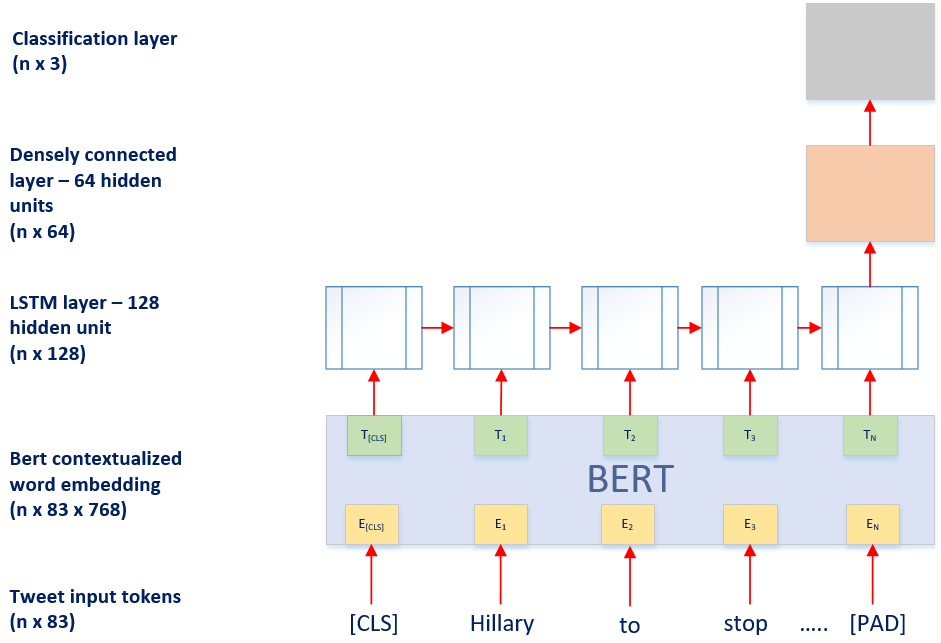
\includegraphics[width=4,height=4]{images/Dessouky_Spittle_Model_Diagram} 

}

\caption{\label{fig:model_diagram}Model Diagram}\label{fig:model_diagram_chunk}
\end{figure}

As previously mentioned, we expect a model that has the capacity to
capture the unique rhetoric seen in tweets to perform well in stance
classification. The combined use of BERT with a LSTM layer would provide
the infrastructure suitable to capture the nuances of hashtags, sarcasm,
and irony frequently used on Twitter.

\hypertarget{hyperparameter-tuning}{%
\subsection{Hyperparameter Tuning}\label{hyperparameter-tuning}}

Since independent models were trained for each of the five topics, we
tuned the model's hyperparameters on a single topic, Hillary Clinton,
and then applied the results to the remaining topics. Hillary Clinton
was selected because it contained the most consistent balance of classes
within both the training and test sets. In addition, its majority class
was the `AGAINST' stance label, which was consistent with all the other
topics, excluding Climate Change. Our overall approach for
hyperparameter tuning was trial and error.
\autoref{fig:hyperparam_table} below details the hyperparameters we
focused on as well as the final value implemented in our models.

\begin{longtable}[]{@{}ll@{}}
\caption{\label{fig:hyperparam_table} Hyperparameters tuned and final
values used}\tabularnewline
\toprule
Hyperparameter & Final Value\tabularnewline
\midrule
\endfirsthead
\toprule
Hyperparameter & Final Value\tabularnewline
\midrule
\endhead
Learning Rate & 0.001\tabularnewline
Epochs & 20\tabularnewline
Dropout Rate & 50\%\tabularnewline
Batch Size & 32\tabularnewline
\# of Bert Fine Tune Layers & 6 layers\tabularnewline
Tweet Pre-processing & None\tabularnewline
\bottomrule
\end{longtable}

Note we ran our model both with tweets pre-processed (all words
lower-cased and punctuation and digits removed) as well as without
pre-processing. The model performed consistently better without
pre-processing applied, and thus, we elected to train all topic models
on the raw tweets.

\hypertarget{training}{%
\subsection{Training}\label{training}}

As mentioned above, we leveraged a batch size of 32 tweets for training.
Adam optimization with a learning rate of 0.001 was used with
categorical cross entropy loss. We used 20 epochs for training on all
topics, except for Climate Change. Climate Change had a considerably
smaller sample size, and thus, required fewer epochs (7 epochs) before
overfitting the model to the training data. Since no development data
was provided, we carved out 15\% of the training data to use as
development data to determine whether we were overfitting during
training. The pre-trained Bert weights were also fine-tuned during
training.

\hypertarget{results}{%
\section{Results}\label{results}}

Our model's results are summarized in the tables below.
\emph{\autoref{fig:classreport_table}} shows the classification report
for our model across all targets. \emph{\autoref{fig:f1rank_table}}
shows the final ranking of our model in the context of the competing
teams in the SemEval-2016 conference, the baseline and updated SVM
models from \emph{Mohammad et al. (2016b) and
}@sobhani-etal-2016-detecting,\_ and the succeeding work by \emph{Sun}
and \emph{Du}. \emph{\autoref{fig:f1all_table}} shows our F1 scores for
each topic in comparison to all teams that achieved a high score in at
least 1 topic as well as the SVM baseline, \emph{Sun et. al}, and
\emph{Du et. al}.

\begin{longtable}[]{@{}lccc@{}}
\caption{\label{fig:classreport_table} Classification
Report}\tabularnewline
\toprule
Stance & Precision & Recall & F1 Score\tabularnewline
\midrule
\endfirsthead
\toprule
Stance & Precision & Recall & F1 Score\tabularnewline
\midrule
\endhead
Against & 81.73 & 67.55 & 73.97\tabularnewline
None & 50.34 & 64.78 & 56.65\tabularnewline
Favor & 60.22 & 71.71 & 65.47\tabularnewline
\bottomrule
\end{longtable}

\begin{longtable}[]{@{}lccc@{}}
\caption{\label{fig:f1rank_table} Final F1 Scores with
Ranks}\tabularnewline
\toprule
Topic & F1 Score & SemEval-2016 Rank & Overall Rank\tabularnewline
\midrule
\endfirsthead
\toprule
Topic & F1 Score & SemEval-2016 Rank & Overall Rank\tabularnewline
\midrule
\endhead
Overall F-macroT & 60.88 & 1 & 2\tabularnewline
Overall F-microT & 69.72 & 1 & 3\tabularnewline
Atheism & 69.66 & 1 & 2\tabularnewline
Hillary Clinton & 64.48 & 2 & 3\tabularnewline
Abortion & 64.06 & 1 & 3\tabularnewline
Climate Change & 48.47 & 3 & 5\tabularnewline
Feminism & 57.76 & 2 & 3\tabularnewline
\bottomrule
\end{longtable}

\begin{longtable}[]{@{}lccccccc@{}}
\caption{\label{fig:f1all_table} F1 Scores for all state-of-the-art
models}\tabularnewline
\toprule
\begin{minipage}[b]{0.22\columnwidth}\raggedright
Team\strut
\end{minipage} & \begin{minipage}[b]{0.10\columnwidth}\centering
Overall (F-microT)\strut
\end{minipage} & \begin{minipage}[b]{0.11\columnwidth}\centering
Overall (F-macroT)\strut
\end{minipage} & \begin{minipage}[b]{0.07\columnwidth}\centering
Atheism\strut
\end{minipage} & \begin{minipage}[b]{0.07\columnwidth}\centering
Climate\strut
\end{minipage} & \begin{minipage}[b]{0.07\columnwidth}\centering
Feminism\strut
\end{minipage} & \begin{minipage}[b]{0.07\columnwidth}\centering
Hillary\strut
\end{minipage} & \begin{minipage}[b]{0.07\columnwidth}\centering
Abortion\strut
\end{minipage}\tabularnewline
\midrule
\endfirsthead
\toprule
\begin{minipage}[b]{0.22\columnwidth}\raggedright
Team\strut
\end{minipage} & \begin{minipage}[b]{0.10\columnwidth}\centering
Overall (F-microT)\strut
\end{minipage} & \begin{minipage}[b]{0.11\columnwidth}\centering
Overall (F-macroT)\strut
\end{minipage} & \begin{minipage}[b]{0.07\columnwidth}\centering
Atheism\strut
\end{minipage} & \begin{minipage}[b]{0.07\columnwidth}\centering
Climate\strut
\end{minipage} & \begin{minipage}[b]{0.07\columnwidth}\centering
Feminism\strut
\end{minipage} & \begin{minipage}[b]{0.07\columnwidth}\centering
Hillary\strut
\end{minipage} & \begin{minipage}[b]{0.07\columnwidth}\centering
Abortion\strut
\end{minipage}\tabularnewline
\midrule
\endhead
\begin{minipage}[t]{0.22\columnwidth}\raggedright
Muhammed et. al\strut
\end{minipage} & \begin{minipage}[t]{0.10\columnwidth}\centering
\textbf{70.32}\strut
\end{minipage} & \begin{minipage}[t]{0.11\columnwidth}\centering
59.01\strut
\end{minipage} & \begin{minipage}[t]{0.07\columnwidth}\centering
69.19\strut
\end{minipage} & \begin{minipage}[t]{0.07\columnwidth}\centering
43.80\strut
\end{minipage} & \begin{minipage}[t]{0.07\columnwidth}\centering
58.72\strut
\end{minipage} & \begin{minipage}[t]{0.07\columnwidth}\centering
61.74\strut
\end{minipage} & \begin{minipage}[t]{0.07\columnwidth}\centering
\textbf{66.91}\strut
\end{minipage}\tabularnewline
\begin{minipage}[t]{0.22\columnwidth}\raggedright
Sun\strut
\end{minipage} & \begin{minipage}[t]{0.10\columnwidth}\centering
69.79\strut
\end{minipage} & \begin{minipage}[t]{0.11\columnwidth}\centering
\textbf{61.00}\strut
\end{minipage} & \begin{minipage}[t]{0.07\columnwidth}\centering
\textbf{70.53}\strut
\end{minipage} & \begin{minipage}[t]{0.07\columnwidth}\centering
49.56\strut
\end{minipage} & \begin{minipage}[t]{0.07\columnwidth}\centering
57.50\strut
\end{minipage} & \begin{minipage}[t]{0.07\columnwidth}\centering
61.84\strut
\end{minipage} & \begin{minipage}[t]{0.07\columnwidth}\centering
66.16\strut
\end{minipage}\tabularnewline
\begin{minipage}[t]{0.22\columnwidth}\raggedright
\textbf{Dessouky \& Spittle}\strut
\end{minipage} & \begin{minipage}[t]{0.10\columnwidth}\centering
69.72\strut
\end{minipage} & \begin{minipage}[t]{0.11\columnwidth}\centering
60.88\strut
\end{minipage} & \begin{minipage}[t]{0.07\columnwidth}\centering
69.66\strut
\end{minipage} & \begin{minipage}[t]{0.07\columnwidth}\centering
48.47\strut
\end{minipage} & \begin{minipage}[t]{0.07\columnwidth}\centering
57.76\strut
\end{minipage} & \begin{minipage}[t]{0.07\columnwidth}\centering
64.48\strut
\end{minipage} & \begin{minipage}[t]{0.07\columnwidth}\centering
64.06\strut
\end{minipage}\tabularnewline
\begin{minipage}[t]{0.22\columnwidth}\raggedright
Du\strut
\end{minipage} & \begin{minipage}[t]{0.10\columnwidth}\centering
68.79\strut
\end{minipage} & \begin{minipage}[t]{0.11\columnwidth}\centering
59.56\strut
\end{minipage} & \begin{minipage}[t]{0.07\columnwidth}\centering
59.77\strut
\end{minipage} & \begin{minipage}[t]{0.07\columnwidth}\centering
\textbf{53.59}\strut
\end{minipage} & \begin{minipage}[t]{0.07\columnwidth}\centering
55.77\strut
\end{minipage} & \begin{minipage}[t]{0.07\columnwidth}\centering
65.38\strut
\end{minipage} & \begin{minipage}[t]{0.07\columnwidth}\centering
63.72\strut
\end{minipage}\tabularnewline
\begin{minipage}[t]{0.22\columnwidth}\raggedright
MITRE\strut
\end{minipage} & \begin{minipage}[t]{0.10\columnwidth}\centering
67.82\strut
\end{minipage} & \begin{minipage}[t]{0.11\columnwidth}\centering
56.03\strut
\end{minipage} & \begin{minipage}[t]{0.07\columnwidth}\centering
61.47\strut
\end{minipage} & \begin{minipage}[t]{0.07\columnwidth}\centering
41.63\strut
\end{minipage} & \begin{minipage}[t]{0.07\columnwidth}\centering
\textbf{62.09}\strut
\end{minipage} & \begin{minipage}[t]{0.07\columnwidth}\centering
57.67\strut
\end{minipage} & \begin{minipage}[t]{0.07\columnwidth}\centering
57.28\strut
\end{minipage}\tabularnewline
\begin{minipage}[t]{0.22\columnwidth}\raggedright
pkudblab\strut
\end{minipage} & \begin{minipage}[t]{0.10\columnwidth}\centering
67.33\strut
\end{minipage} & \begin{minipage}[t]{0.11\columnwidth}\centering
58.57\strut
\end{minipage} & \begin{minipage}[t]{0.07\columnwidth}\centering
63.34\strut
\end{minipage} & \begin{minipage}[t]{0.07\columnwidth}\centering
52.69\strut
\end{minipage} & \begin{minipage}[t]{0.07\columnwidth}\centering
51.33\strut
\end{minipage} & \begin{minipage}[t]{0.07\columnwidth}\centering
64.41\strut
\end{minipage} & \begin{minipage}[t]{0.07\columnwidth}\centering
61.09\strut
\end{minipage}\tabularnewline
\begin{minipage}[t]{0.22\columnwidth}\raggedright
TakeLab\strut
\end{minipage} & \begin{minipage}[t]{0.10\columnwidth}\centering
66.83\strut
\end{minipage} & \begin{minipage}[t]{0.11\columnwidth}\centering
58.00\strut
\end{minipage} & \begin{minipage}[t]{0.07\columnwidth}\centering
67.25\strut
\end{minipage} & \begin{minipage}[t]{0.07\columnwidth}\centering
41.25\strut
\end{minipage} & \begin{minipage}[t]{0.07\columnwidth}\centering
53.01\strut
\end{minipage} & \begin{minipage}[t]{0.07\columnwidth}\centering
\textbf{67.12}\strut
\end{minipage} & \begin{minipage}[t]{0.07\columnwidth}\centering
61.38\strut
\end{minipage}\tabularnewline
\begin{minipage}[t]{0.22\columnwidth}\raggedright
Majority Class\strut
\end{minipage} & \begin{minipage}[t]{0.10\columnwidth}\centering
65.22\strut
\end{minipage} & \begin{minipage}[t]{0.11\columnwidth}\centering
40.09\strut
\end{minipage} & \begin{minipage}[t]{0.07\columnwidth}\centering
42.11\strut
\end{minipage} & \begin{minipage}[t]{0.07\columnwidth}\centering
42.12\strut
\end{minipage} & \begin{minipage}[t]{0.07\columnwidth}\centering
39.10\strut
\end{minipage} & \begin{minipage}[t]{0.07\columnwidth}\centering
36.83\strut
\end{minipage} & \begin{minipage}[t]{0.07\columnwidth}\centering
40.30\strut
\end{minipage}\tabularnewline
\begin{minipage}[t]{0.22\columnwidth}\raggedright
DeepStance\strut
\end{minipage} & \begin{minipage}[t]{0.10\columnwidth}\centering
63.54\strut
\end{minipage} & \begin{minipage}[t]{0.11\columnwidth}\centering
52.86\strut
\end{minipage} & \begin{minipage}[t]{0.07\columnwidth}\centering
52.90\strut
\end{minipage} & \begin{minipage}[t]{0.07\columnwidth}\centering
40.40\strut
\end{minipage} & \begin{minipage}[t]{0.07\columnwidth}\centering
52.34\strut
\end{minipage} & \begin{minipage}[t]{0.07\columnwidth}\centering
55.35\strut
\end{minipage} & \begin{minipage}[t]{0.07\columnwidth}\centering
63.32\strut
\end{minipage}\tabularnewline
\begin{minipage}[t]{0.22\columnwidth}\raggedright
\href{mailto:IDI@NTNU}{\nolinkurl{IDI@NTNU}}\strut
\end{minipage} & \begin{minipage}[t]{0.10\columnwidth}\centering
62.47\strut
\end{minipage} & \begin{minipage}[t]{0.11\columnwidth}\centering
55.08\strut
\end{minipage} & \begin{minipage}[t]{0.07\columnwidth}\centering
59.59\strut
\end{minipage} & \begin{minipage}[t]{0.07\columnwidth}\centering
54.86\strut
\end{minipage} & \begin{minipage}[t]{0.07\columnwidth}\centering
48.59\strut
\end{minipage} & \begin{minipage}[t]{0.07\columnwidth}\centering
57.89\strut
\end{minipage} & \begin{minipage}[t]{0.07\columnwidth}\centering
54.47\strut
\end{minipage}\tabularnewline
\bottomrule
\end{longtable}

The results in the above tables demonstrate the strength of our model.
When comparing against teams participating in the SemEval2016
competition (see \emph{Table 4}, column \emph{SemEval-2016 Rank}), we
achieved the highest overall micro F1 and macro F1 scores. We also
achieved the top F1 score in the Atheism and Abortion topics, while
finishing second in Hillary Clinton and Feminism, and third in Climate
Change. When including \emph{Sun et. al} and \emph{Du et. al}'s
post-conference contributions as well as the SVM baseline, we do not
have any top scores (see \emph{Table 4}, column \emph{Overall Rank}).
However, we still achieved the second highest macro F1 score, trailing
\emph{Sun et. al} by only 0.12 (see \emph{Table 5}). We also achieved
the third highest micro F1 score, behind \emph{Sun et. al} and
\emph{Muhammed et. al}. Note that micro F1 score tends to be higher for
models that perform better on the majority class, while macro F1 score
tends to be higher for models that perform well on all classes. This can
be seen in the comparison between the majority classifier's micro and
macro F1 scores. The majority classifier scores a 65.22 on micro F1
score, but only 40.09 on macro F1. Our model achieved universally higher
results than the majority classifier. See
\emph{\autoref{fig:versus_majority}}.

\begin{figure}

{\centering \includegraphics{StanceDetectionTweets_DessoukySpittle_files/figure-latex/plot_versus_majority-1} 

}

\caption{\label{fig:versus_majority}Results versus Majority Classifier}\label{fig:plot_versus_majority}
\end{figure}

\newpage

\hypertarget{limitations}{%
\section{Limitations}\label{limitations}}

While we were able to build an effective model for stance detection, we
came across a number of apparent limitations. First, as mentioned within
the \textbf{Data, Task, and Evaluation} section, the key query hashtags
were removed from the training and test data, which would have been
incredibly valuable in determining stance in the real world. Next, the
stance labels were highly skewed. \emph{\autoref(fig:data\_dst)} below
shows the distribution of the labels for each target. While we allocated
higher weights to the minority classes during the training process, our
model still proved to be much more effective in predicting the majority
class versus the minority classes.

\begin{longtable}[]{@{}lccccccccc@{}}
\caption{\label{fig:data_dst} Data distribution}\tabularnewline
\toprule
\begin{minipage}[b]{0.15\columnwidth}\raggedright
Target\strut
\end{minipage} & \begin{minipage}[b]{0.07\columnwidth}\centering
\# total\strut
\end{minipage} & \begin{minipage}[b]{0.07\columnwidth}\centering
\# train\strut
\end{minipage} & \begin{minipage}[b]{0.07\columnwidth}\centering
favor (\% of train)\strut
\end{minipage} & \begin{minipage}[b]{0.07\columnwidth}\centering
none (\% of train)\strut
\end{minipage} & \begin{minipage}[b]{0.07\columnwidth}\centering
against (\% of train)\strut
\end{minipage} & \begin{minipage}[b]{0.07\columnwidth}\centering
\# test\strut
\end{minipage} & \begin{minipage}[b]{0.07\columnwidth}\centering
favor (\% of test)\strut
\end{minipage} & \begin{minipage}[b]{0.07\columnwidth}\centering
none (\% of test)\strut
\end{minipage} & \begin{minipage}[b]{0.07\columnwidth}\centering
against (\% of test\strut
\end{minipage}\tabularnewline
\midrule
\endfirsthead
\toprule
\begin{minipage}[b]{0.15\columnwidth}\raggedright
Target\strut
\end{minipage} & \begin{minipage}[b]{0.07\columnwidth}\centering
\# total\strut
\end{minipage} & \begin{minipage}[b]{0.07\columnwidth}\centering
\# train\strut
\end{minipage} & \begin{minipage}[b]{0.07\columnwidth}\centering
favor (\% of train)\strut
\end{minipage} & \begin{minipage}[b]{0.07\columnwidth}\centering
none (\% of train)\strut
\end{minipage} & \begin{minipage}[b]{0.07\columnwidth}\centering
against (\% of train)\strut
\end{minipage} & \begin{minipage}[b]{0.07\columnwidth}\centering
\# test\strut
\end{minipage} & \begin{minipage}[b]{0.07\columnwidth}\centering
favor (\% of test)\strut
\end{minipage} & \begin{minipage}[b]{0.07\columnwidth}\centering
none (\% of test)\strut
\end{minipage} & \begin{minipage}[b]{0.07\columnwidth}\centering
against (\% of test\strut
\end{minipage}\tabularnewline
\midrule
\endhead
\begin{minipage}[t]{0.15\columnwidth}\raggedright
Atheism\strut
\end{minipage} & \begin{minipage}[t]{0.07\columnwidth}\centering
733\strut
\end{minipage} & \begin{minipage}[t]{0.07\columnwidth}\centering
513\strut
\end{minipage} & \begin{minipage}[t]{0.07\columnwidth}\centering
17.9\strut
\end{minipage} & \begin{minipage}[t]{0.07\columnwidth}\centering
59.3\strut
\end{minipage} & \begin{minipage}[t]{0.07\columnwidth}\centering
22.8\strut
\end{minipage} & \begin{minipage}[t]{0.07\columnwidth}\centering
220\strut
\end{minipage} & \begin{minipage}[t]{0.07\columnwidth}\centering
14.5\strut
\end{minipage} & \begin{minipage}[t]{0.07\columnwidth}\centering
72.7\strut
\end{minipage} & \begin{minipage}[t]{0.07\columnwidth}\centering
12.7\strut
\end{minipage}\tabularnewline
\begin{minipage}[t]{0.15\columnwidth}\raggedright
Climate Change\strut
\end{minipage} & \begin{minipage}[t]{0.07\columnwidth}\centering
564\strut
\end{minipage} & \begin{minipage}[t]{0.07\columnwidth}\centering
395\strut
\end{minipage} & \begin{minipage}[t]{0.07\columnwidth}\centering
53.7\strut
\end{minipage} & \begin{minipage}[t]{0.07\columnwidth}\centering
3.8\strut
\end{minipage} & \begin{minipage}[t]{0.07\columnwidth}\centering
42.5\strut
\end{minipage} & \begin{minipage}[t]{0.07\columnwidth}\centering
169\strut
\end{minipage} & \begin{minipage}[t]{0.07\columnwidth}\centering
72.8\strut
\end{minipage} & \begin{minipage}[t]{0.07\columnwidth}\centering
6.5\strut
\end{minipage} & \begin{minipage}[t]{0.07\columnwidth}\centering
20.7\strut
\end{minipage}\tabularnewline
\begin{minipage}[t]{0.15\columnwidth}\raggedright
Feminist Movement\strut
\end{minipage} & \begin{minipage}[t]{0.07\columnwidth}\centering
949\strut
\end{minipage} & \begin{minipage}[t]{0.07\columnwidth}\centering
664\strut
\end{minipage} & \begin{minipage}[t]{0.07\columnwidth}\centering
31.6\strut
\end{minipage} & \begin{minipage}[t]{0.07\columnwidth}\centering
49.4\strut
\end{minipage} & \begin{minipage}[t]{0.07\columnwidth}\centering
19.0\strut
\end{minipage} & \begin{minipage}[t]{0.07\columnwidth}\centering
285\strut
\end{minipage} & \begin{minipage}[t]{0.07\columnwidth}\centering
20.4\strut
\end{minipage} & \begin{minipage}[t]{0.07\columnwidth}\centering
64.2\strut
\end{minipage} & \begin{minipage}[t]{0.07\columnwidth}\centering
15.4\strut
\end{minipage}\tabularnewline
\begin{minipage}[t]{0.15\columnwidth}\raggedright
Hillary Clinton\strut
\end{minipage} & \begin{minipage}[t]{0.07\columnwidth}\centering
984\strut
\end{minipage} & \begin{minipage}[t]{0.07\columnwidth}\centering
689\strut
\end{minipage} & \begin{minipage}[t]{0.07\columnwidth}\centering
17.1\strut
\end{minipage} & \begin{minipage}[t]{0.07\columnwidth}\centering
57.0\strut
\end{minipage} & \begin{minipage}[t]{0.07\columnwidth}\centering
25.8\strut
\end{minipage} & \begin{minipage}[t]{0.07\columnwidth}\centering
295\strut
\end{minipage} & \begin{minipage}[t]{0.07\columnwidth}\centering
15.3\strut
\end{minipage} & \begin{minipage}[t]{0.07\columnwidth}\centering
58.3\strut
\end{minipage} & \begin{minipage}[t]{0.07\columnwidth}\centering
26.4\strut
\end{minipage}\tabularnewline
\begin{minipage}[t]{0.15\columnwidth}\raggedright
Legalization of Abortion\strut
\end{minipage} & \begin{minipage}[t]{0.07\columnwidth}\centering
933\strut
\end{minipage} & \begin{minipage}[t]{0.07\columnwidth}\centering
653\strut
\end{minipage} & \begin{minipage}[t]{0.07\columnwidth}\centering
18.5\strut
\end{minipage} & \begin{minipage}[t]{0.07\columnwidth}\centering
54.4\strut
\end{minipage} & \begin{minipage}[t]{0.07\columnwidth}\centering
27.1\strut
\end{minipage} & \begin{minipage}[t]{0.07\columnwidth}\centering
280\strut
\end{minipage} & \begin{minipage}[t]{0.07\columnwidth}\centering
16.4\strut
\end{minipage} & \begin{minipage}[t]{0.07\columnwidth}\centering
57.3\strut
\end{minipage} & \begin{minipage}[t]{0.07\columnwidth}\centering
18.4\strut
\end{minipage}\tabularnewline
\bottomrule
\end{longtable}

In addition, there was a high level of disagreement amongst the label
`encoders', which translates to a higher expected error rate in our
model. We can expect our model to struggle classifying the stance of
tweets in which humans do not consistently agree. Further, the total
number of tweets in our dataset was low for a NLP problem. This may
affect the reproducibility of our model results. Re-running the same
model on the identical training and test sets would produce slightly
different results, despite fitting the training data to near 100\%
accuracy.

\hypertarget{error-analysis}{%
\subsection{Error Analysis}\label{error-analysis}}

\emph{\autoref{fig:confusion_matrix}} presents a confusion matrix
detailing the distribution of predicted versus true labels for our
model. Given that the Against stance is the majority class, it is no
surprise that the largest contributors to errors are false-negative
Against observations.

Errors for target \textbf{Atheism} were manually reviewed by the authors
to better understand the natures of mis-classified tweets. Error tweets
were categorized according to whether the purported ``true'' label or
the predicted label from our model appeared to be correct (or if neither
appeared correct). \autoref{fig:error_analysis} below shows the result
of this error review and annotation.

\begin{figure}

{\centering \includegraphics{StanceDetectionTweets_DessoukySpittle_files/figure-latex/confusion_matrix_chunk-1} 

}

\caption{\label{fig:confusion_matrix}Confusion Matrix}\label{fig:confusion_matrix_chunk}
\end{figure}

\begin{figure}

{\centering \includegraphics{StanceDetectionTweets_DessoukySpittle_files/figure-latex/error_analysis_chunk-1} 

}

\caption{\label{fig:error_analysis}Atheism Error Analysis Summary of Issues}\label{fig:error_analysis_chunk}
\end{figure}

It was surprising how many tweets appeared to have been assigned the
incorrect true label. To be clear, there is a substantial amount of
ambiguity in these tweets (as has been mentioned, there was a high
degree of disagreement among encoders), but we will detail different
types of mis-labeled tweets to highlight where and how we think encoders
were mistaken.

First and foremost, some tweet ``true'' labels were blatantly and
unambiguously wrong.

\begin{quote}
\textbf{Topic}: Atheism \textbar{} \textbf{True Label}: Against
\textbar{} \textbf{Predicted Label}: Favor \textbar{} \textbf{Correct}:
Favor\\
RT {[}AT{]}br\_holden: Atheists have every right to exist in the public
sphere. \#freethinker \#SemST
\end{quote}

The above tweet positively discusses the target directly
(atheists/atheism) and even uses a hashtag that is clearly opposed to
religion (and therefore aligned with atheism).

Other true label error examples have common challenges with the tweet
text that may have caused some of these errors in annotation. Generally,
ambiguous texts suffer from some form of lack of context.

\emph{Missing Context} errors occur when certain tweets reference very
specific people or things that may be hard to align with the target or
require a leap in assumption about connection of target.

\begin{quote}
\textbf{Topic}: Atheism \textbar{} \textbf{True Label}: Against
\textbar{} \textbf{Predicted Label}: Favor \textbar{} \textbf{Correct}:
Favor\\
Next time you hear someone say that our Founding Fathers intended a
``Christian Nation,'' show 'em those quotes. \#SemST
\end{quote}

The above tweet, for example, references ``those quotes'' which we do
not see, therefore we cannot make a judgment as to how ``showing 'em the
quotes'' would align with the target.

Similarly, \emph{Referential} errors occur when other tweets refernce a
target other than the target of interest and an unreasonable leap in
assumption is made to come to a conclusion on that author's potential
stance on the target.

\begin{quote}
\textbf{Topic}: Atheism \textbar{} \textbf{True Label}: Against
\textbar{} \textbf{Predicted Label}: Neither \textbar{}
\textbf{Correct}: Neither\\
Happy Independence Day to America and her beautiful constitution
\#IndependenceDay \#USA \#SemST
\end{quote}

It is notable in the above tweet that the query hashtag, which is not
presented, could be the point that makes the author's stance clear.
However, without it, it is not reasonable to draw the conclusion that
celebrating Independence Day and the constitution exhibits a stance
Against Atheism.

Lastly, a common problem in sentiment analysis is \emph{Sarcsm}.

\begin{quote}
\textbf{Topic}: Atheism \textbar{} \textbf{True Label}: Against
\textbar{} \textbf{Predicted Label}: Favor \textbar{} \textbf{Correct}:
Favor\\
Phew! Am glad we came to our senses and worship a 2,000 year old
carpenter. - Bart Simpson \#jokes \#SemST
\end{quote}

\begin{quote}
\textbf{Topic}: Atheism \textbar{} \textbf{True Label}: Against
\textbar{} \textbf{Predicted Label}: Favor \textbar{} \textbf{Correct}:
Against\\
{[}AT{]}Ageoftheatheist \textasciitilde{} ``Age of the \#Atheist'' where
life has no purpose \& no hope! \#SemST
\end{quote}

The above two example tweets (which exhibit both mis-labeled data and an
error of our model's prediction) are very clearly joking/mocking.

This apparent mis-labeling obviously causes some concern about the
ability to train a model consistently that performs well on unseen data.
However, the majority of instances reviewed where our model made obvious
mistakes were very clearly incorrect predictions. There were no
systematic issues. It is notable that our model made consistent errors
across true label categories, however the annotaters made errors almost
exclusively in the majority Against stance. The against stance
constitutees 73\% of test set data observations for the atheism target,
indicating that some amount of the errors may be attributable to
fatigue, perhaps, or some factor that causes repeated annotation to lean
toward the majority class.

\hypertarget{conclusion-and-future-work}{%
\section{Conclusion and Future Work}\label{conclusion-and-future-work}}

In this paper, we implement BERT for contextualized word embeddings in a
neural network model used to effectively detect stance. We propose a
novel model architecture for use on the SemEval-2016 Task 6 dataset.
While we did not beat the current top score, we obtained results in line
with several of the state-of-the-art models. We achieved a F-microT of
69.72 and a F-macroT of 60.88, which ranked 3rd and 2nd, respectively,
amongst all contributors to the task. This demonstrates the potential
BERT has as a method of obtaining contextualized word embeddings for the
purpose of stance classification.

Going forward, there are a couple additional areas in which there is
room for improvement. First, we would like to explore the use of a
bidirectional LSTM layer in lieu of the current LSTM layer implemented
in our model. In addition, we would like to investigate the benefits of
using BERT Large in the embedding layer in place of BERT Base.

Another potential area for improvement is training BERT from scratch
rather than leveraging the pre-trained weights and subsequently
fine-tuning with the SemEval-2016 Task 6 data. If a large corpus could
be obtained similar to that described in the \textbf{Data, Task, and
Evaluation} section above, training BERT from scratch would likely
result in a significant boost in F1 score. Lastly, given the small data
set size and high skewness, putting effort into collecting more data to
increase the sample size and balance out the classes would likely
benefit the model performance.

\newpage

\hypertarget{references}{%
\section*{References}\label{references}}
\addcontentsline{toc}{section}{References}

\hypertarget{refs}{}
\leavevmode\hypertarget{ref-bohler-etal-2016-idi}{}%
Bøhler, Henrik, Petter Asla, Erwin Marsi, and Rune Sætre. 2016.
``IDI@NTNU at SemEval-2016 Task 6: Detecting Stance in Tweets Using
Shallow Features and GloVe Vectors for Word Representation.'' In
\emph{Proceedings of the 10th International Workshop on Semantic
Evaluation (SemEval-2016)}, 445--50. San Diego, California: Association
for Computational Linguistics.
\url{https://doi.org/10.18653/v1/S16-1072}.

\leavevmode\hypertarget{ref-ijcai2017-557}{}%
Du, Jiachen, Ruifeng Xu, Yulan He, and Lin Gui. 2017. ``Stance
Classification with Target-Specific Neural Attention.'' In
\emph{Proceedings of the Twenty-Sixth International Joint Conference on
Artificial Intelligence, IJCAI-17}, 3988--94.
\url{https://doi.org/10.24963/ijcai.2017/557}.

\leavevmode\hypertarget{ref-ma-unpublished}{}%
Ma, Guoqin. 2019. ``Tweets Classification with Bert in the Field of
Disaster Management.''

\leavevmode\hypertarget{ref-mayfield-black-2019-stance}{}%
Mayfield, Elijah, and Alan Black. 2019. ``Stance Classification, Outcome
Prediction, and Impact Assessment: NLP Tasks for Studying Group
Decision-Making.'' In \emph{Proceedings of the Third Workshop on Natural
Language Processing and Computational Social Science}, 65--77.
Minneapolis, Minnesota: Association for Computational Linguistics.
\url{https://doi.org/10.18653/v1/W19-2108}.

\leavevmode\hypertarget{ref-mohammad-etal-2016-dataset}{}%
Mohammad, Saif, Svetlana Kiritchenko, Parinaz Sobhani, Xiaodan Zhu, and
Colin Cherry. 2016a. ``A Dataset for Detecting Stance in Tweets.'' In
\emph{Proceedings of the Tenth International Conference on Language
Resources and Evaluation (LREC'16)}, 3945--52. Portorož, Slovenia:
European Language Resources Association (ELRA).
\url{https://www.aclweb.org/anthology/L16-1623}.

\leavevmode\hypertarget{ref-mohammad-etal-2016-semeval}{}%
---------. 2016b. ``SemEval-2016 Task 6: Detecting Stance in Tweets.''
In \emph{Proceedings of the 10th International Workshop on Semantic
Evaluation (SemEval-2016)}, 31--41. San Diego, California: Association
for Computational Linguistics.
\url{https://doi.org/10.18653/v1/S16-1003}.

\leavevmode\hypertarget{ref-sobhani-etal-2016-detecting}{}%
Sobhani, Parinaz, Saif Mohammad, and Svetlana Kiritchenko. 2016.
``Detecting Stance in Tweets and Analyzing Its Interaction with
Sentiment.'' In \emph{Proceedings of the Fifth Joint Conference on
Lexical and Computational Semantics}, 159--69. Berlin, Germany:
Association for Computational Linguistics.
\url{https://doi.org/10.18653/v1/S16-2021}.

\leavevmode\hypertarget{ref-sun-etal-2018-stance}{}%
Sun, Qingying, Zhongqing Wang, Qiaoming Zhu, and Guodong Zhou. 2018.
``Stance Detection with Hierarchical Attention Network.'' In
\emph{Proceedings of the 27th International Conference on Computational
Linguistics}, 2399--2409. Santa Fe, New Mexico, USA: Association for
Computational Linguistics.
\url{https://www.aclweb.org/anthology/C18-1203}.

\leavevmode\hypertarget{ref-tutek-etal-2016-takelab}{}%
Tutek, Martin, Ivan Sekulić, Paula Gombar, Ivan Paljak, Filip Čulinović,
Filip Boltužić, Mladen Karan, Domagoj Alagić, and Jan Šnajder. 2016.
``TakeLab at SemEval-2016 Task 6: Stance Classification in Tweets Using
a Genetic Algorithm Based Ensemble.'' In \emph{Proceedings of the 10th
International Workshop on Semantic Evaluation (SemEval-2016)}, 464--68.
San Diego, California: Association for Computational Linguistics.
\url{https://doi.org/10.18653/v1/S16-1075}.

\leavevmode\hypertarget{ref-vijayaraghavan-etal-2016-deepstance}{}%
Vijayaraghavan, Prashanth, Ivan Sysoev, Soroush Vosoughi, and Deb Roy.
2016. ``DeepStance at SemEval-2016 Task 6: Detecting Stance in Tweets
Using Character and Word-Level CNNs.'' In \emph{Proceedings of the 10th
International Workshop on Semantic Evaluation (SemEval-2016)}, 413--19.
San Diego, California: Association for Computational Linguistics.
\url{https://doi.org/10.18653/v1/S16-1067}.

\leavevmode\hypertarget{ref-wei-etal-2016-pkudblab}{}%
Wei, Wan, Xiao Zhang, Xuqin Liu, Wei Chen, and Tengjiao Wang. 2016.
``Pkudblab at SemEval-2016 Task 6 : A Specific Convolutional Neural
Network System for Effective Stance Detection.'' In \emph{Proceedings of
the 10th International Workshop on Semantic Evaluation (SemEval-2016)},
384--88. San Diego, California: Association for Computational
Linguistics. \url{https://doi.org/10.18653/v1/S16-1062}.

\leavevmode\hypertarget{ref-zarrella-marsh-2016-mitre}{}%
Zarrella, Guido, and Amy Marsh. 2016. ``MITRE at SemEval-2016 Task 6:
Transfer Learning for Stance Detection.'' In \emph{Proceedings of the
10th International Workshop on Semantic Evaluation (SemEval-2016)},
458--63. San Diego, California: Association for Computational
Linguistics. \url{https://doi.org/10.18653/v1/S16-1074}.


\end{document}
